\chapter*{Android: La Revolución Móvil}

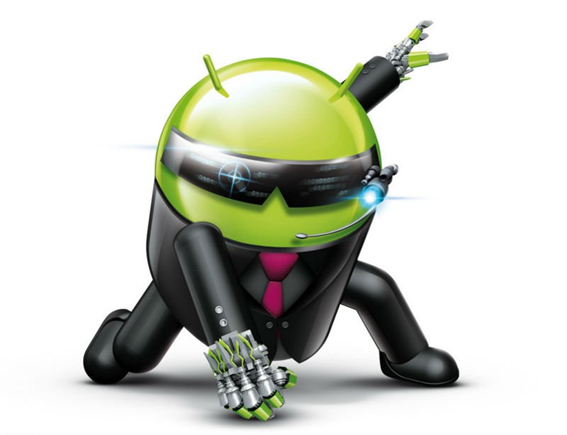
\includegraphics[scale=1]{img/cp05/img0501.png}

Android es un sistema operativo basado en Linux de código abierto, utilizado en dispositivos móviles con pantalla táctil como Smartphones y tablets. El sistema fue 
desarrollado por Android Inc. que Google adquirió en 2005. Android se presentó en 2007 junto con la Open Handset Alliance, un consorcio de compañías de hardware, software y 
telecomunicaciones, cuyo objetivo era avanzar en los estándares de los sistemas abiertos. El primer teléfono con este sistema operativo fue el HTC Dream, que empezó a 
venderse en octubre del 2008. A pesar de su corto tiempo en el mercado, Android se ha posicionado como el sistema operativo número uno en dispositivos móviles por su gran 
variedad de aplicaciones, su funcionalidad y excelente diseño al usuario; además por ser de código abierto es de gran aceptación por la comunidad de desarrolladores que 
disfrutan adaptándolo a su gusto y creando nuevas ROMS. Android cuenta con más de 1 millón de aplicaciones, de donde dos terceras partes son gratuitas y se encuentran en la 
Play Store, ademas de permitirle a los usuarios descargar aplicaciones de otras compañías, detalle que hace de este sistema operativo el de mayor aceptación.


\section*{¿Quién Es El Genio Detrás De Esta Maravilla?}

\includegraphics[scale=1]{img/cp05/img0502.png}

El empresario y desarrollador Andy Rubin bajo la filosofía del Open Source, tuvo la idea de desarrollar un sistema operativo para móviles, el cual llamó Android. Tras 
analizar que la gran fragmentación del mercado hacía imposible que la tecnología evolucionara rápidamente en el sector de los dispositivos móviles; decidió plantear la idea 
de un sistema operativo para celulares que fuera de código abierto y adaptable a cualquier hardware, pero que además ofreciera un entorno de desarrollo libre que permitiera 
crear aplicaciones para este sistema operativo y que corriera en cualquier hardware que lo soportara.

Andy Rubin ya contaba con varios inversionistas que estaban dispuestos a invertir en su proyecto llamado Android, pero tras los rumores de un proyecto similar llamado 
Symbian que también corría sobre Linux, decide acudir a Google para ofrecerles exclusividad en las búsquedas realizadas desde los celulares con Android a cambio de que 
ellos expresaran públicamente su apoyo a la plataforma. Cuando Rubin le hace la presentación al CEO de Google, Larry Page, en 2005, este le ofrece comprar su compañía por 
50 millones de dólares, y la dirección del departamento de la compañía que se encargaría del desarrollo de la plataforma para celulares. En la actualidad Rubin no solo 
supervisa el progreso de Android sino que es también el vicepresidente de ingeniería en Google.

\section*{¡Curiosidades!}
Andy Rubin el creador de Android que ahora hace parte de Google y la fuerte competencia de Apple y Microsoft en cuanto a dispositivos móviles se refiere, trabajo en sus 
inicios como ingeniero de estas dos grandes compañías.

El creador del llamativo logo de Android fue Irina Blok, empresa encargada de crear imágenes comerciales. Irina se inspiró en un personaje de un juego de la videoconsola 
Atari Lynx llamado "Gauntlet: The Third Encounter". "Andy" como decidieron llamar al logo insignia de Android, fue inspirado en la novela de Philip K. Dick ¿Sueñan los 
androides con ovejas eléctricas?; en el libro de habla sobre unos androides llamados Nexus-6, de allí también el nombre de los dispositivos insignia de Google.

El 5 de noviembre es el día del cumpleaños de Android o así es considerado por muchos ya que fue para esa fecha del año 2007 que fue lanzada la versión beta de este sistema 
operativo.

En Android cada una de sus version reciben el nombre de postres en ingles; en cada versión el postre elegido empieza por una letra distinta siguiendo un orden alfabético:

\begin{itemize}
	\item Apple Pie (v1.0), Tarta de manzana.
	\item Banana Bread (v1.1), Pan de plátano.
	\item Cupcake (v1.5), Panque.
	\item Donut (v1.6), Rosquilla.
	\item Éclair (v2.0/v2.1), Pastel francés.
	\item Froyo (v2.2), Yogurt de helado.
	\item Gingerbread (v2.3), Pan de jengibre.
	\item Honeycomb (v3.0/v3.1/v3.2), Panal de miel.
	\item Ice Cream Sandwich (v4.0), Sándwich de helado.
	\item Jelly Bean (v4.1/v4.2/v4.3), Dulces.
	\item KitKat (v4.4). Galleta de Chocolate.
\end{itemize}

\section*{Historia y Características}
Comercialmente android fue lanzado en su primera versión llamada apple pie o Android 1.0 el 23 de septiembre del 2008 y fue el HTC Dream el primer movil con Android en el 
mercado, esta primera versión es considerada la de mayor novedad e incorporaciones en toda la evolución de android pues era la raíz para el comienzo de un sistema operativo 
a nivel comercial. desde ese momento se marcó una gran diferencia en la telefonía movil ya que este sistema operativo trae consigo muchas novedades e incorporaciones de las 
cuales las más destacadas en esta primera versión son:

\begin{itemize}
	\item Incorporación de un mercado para compra y descarga de aplicaciones bajo el nombre de Android Market.
	\item Un navegador web con soporte múltiples ventanas y  capaz de abrir páginas web en HTML y XHTML.
	\item Soporte básico para cámara de fotos.
	\item Posibilidad de crear carpetas e introducir iconos de aplicaciones en ellas desde el escritorio.
	\item Acceder a servidores de correo electrónico por web soportando los protocolos POP3, IMAP4 y SMTP.
	\item Sincronización con los productos de Google: Gmail, Google Calendar y Google Contacts.
	\item Incorporación de productos de Google: GTalk, Google Maps, YouTube, Google Sync y Google Search.
	\item Mensajería instantánea, SMS y MMS.
	\item Reproductor de música (sin soporte para reproducir vídeo).
	\item Soporte para teléfonos con LED.
	\item Notificaciones en la barra de estado con posibilidad de establecer alertas por timbre, LED o vibración.
	\item Marcación por voz.
	\item Soporte para fondos de pantalla y Widgets.
	\item Conectividad para WiFi y Bluetooth.
	\item Incorporación de aplicaciones básicas: Alarma, Ajustes, Calculadora, Dialer, Escritorio y  Galería.
\end{itemize}